\chapter{Two-Dimensional SEAS model}
\label{chap:2DSEAS}

\section{BP1 Benchmark Problem}
Erickson et al proposed the BP1 benchmark problem in \cite{BP1-Benchmark} based on the SEAS model of \cite{GeneralSEASSimulations}, which is a 2D antiplane problem with a 1D vertical fault. It means that the domain represents surface orthogonal to the real fault and only shear stress and displacements out of the plane are considered. A scheme of the model is given in \autoref{fig:2DSEASModel}. Two square, symmetric tectonic plates are pulled in opposite directions by an environment slip rate $V_p/2=5\cdot10^{-10}$m/s, applied as Dirichlet condition on the yellow boundary of the domain. Next, there is no resistance to the tectonic plates at the open surface, it implies Neumann boundary condition which forces the gradient of the displacement to zero. Finally, the most interesting section of the domain is the rate-and-state fault. It is driven by the rate-and-state friction with Dieterich-Ruina ageing described in \autoref{ssec:FrictionLaws} and describes the transition from the bottom of the fault, where the slip increases linearly in time, and the top, which does not move most of the time, recovers the accumulated delay by a sudden increase in slip. \\

\begin{figure}[H]
	\centering
	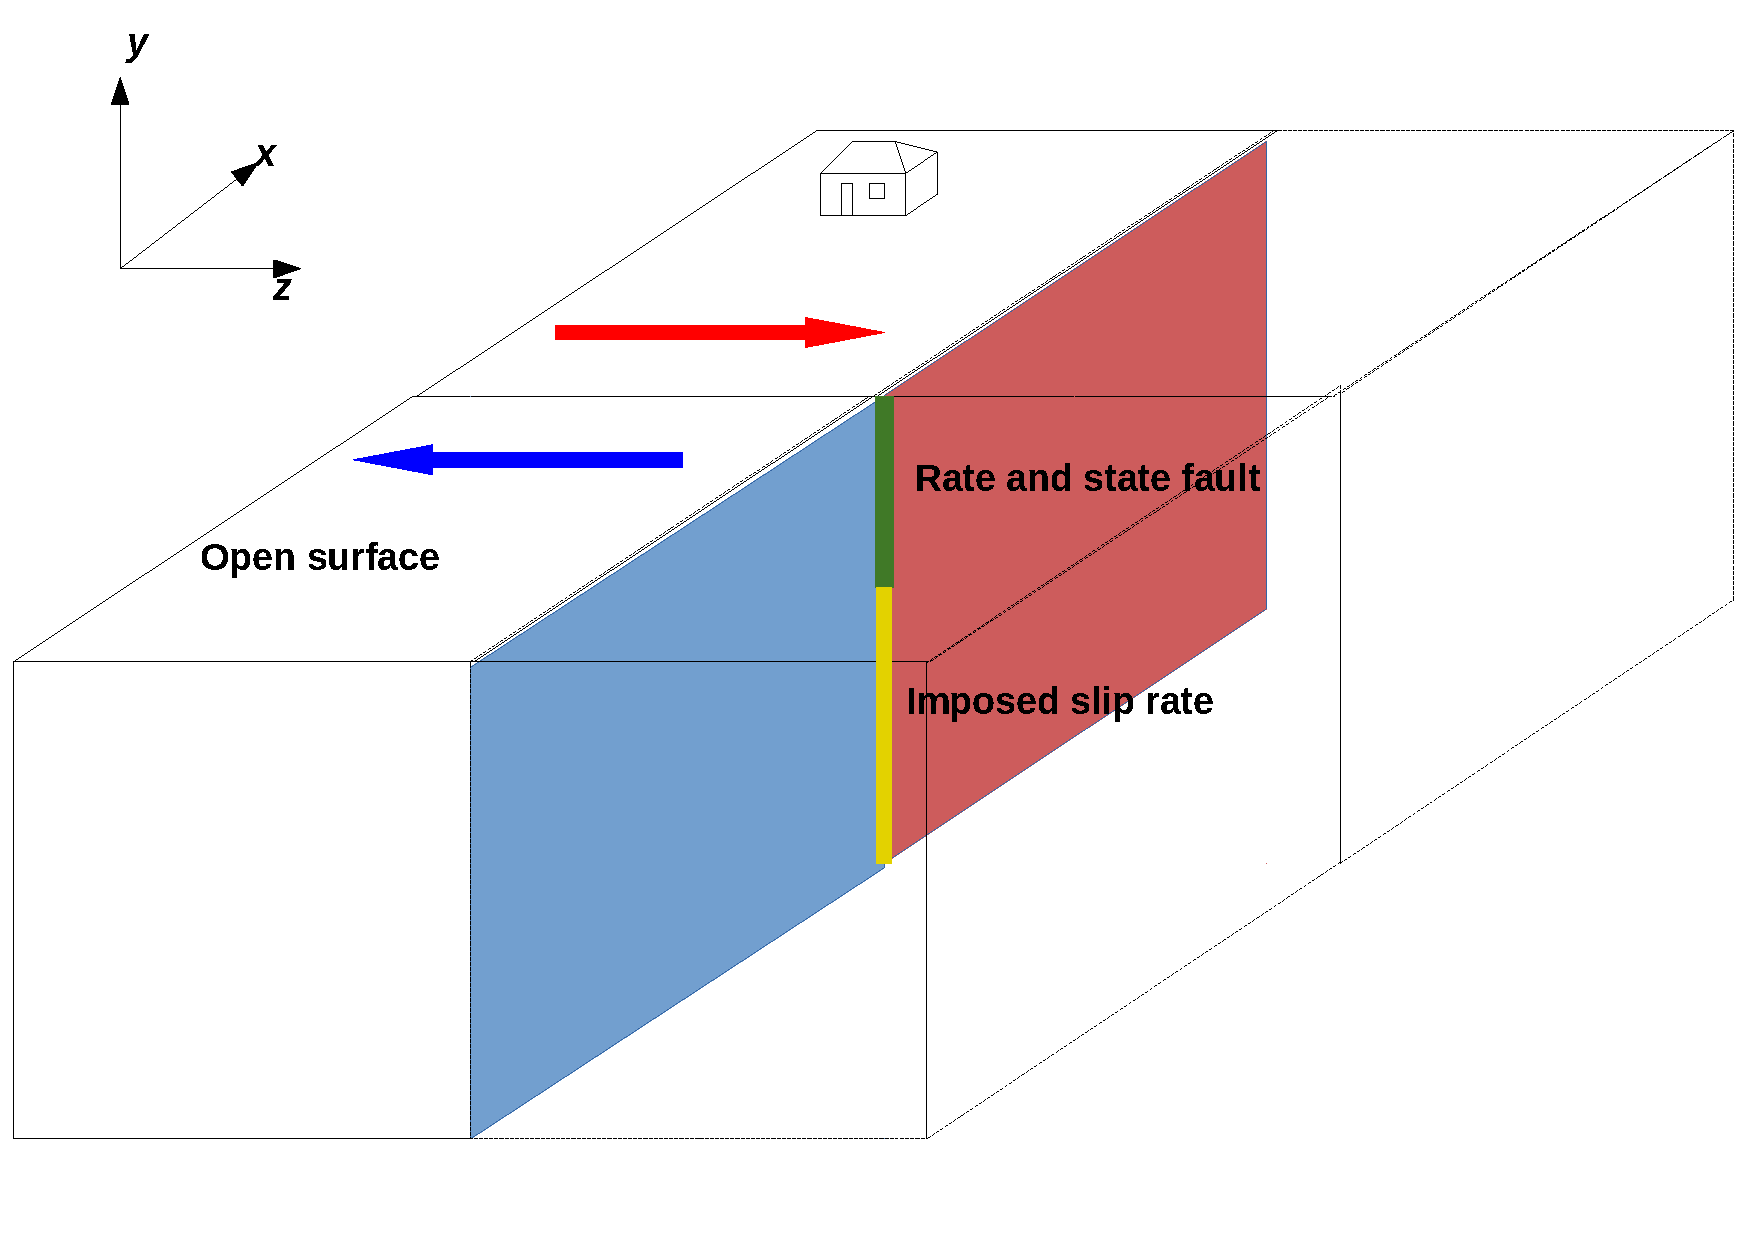
\includegraphics[width=0.4\textwidth]{images/SEAS_2D_picture.pdf}
	\caption{General set-up of the two-dimensional SEAS model}
	\label{fig:2DSEASModel}
\end{figure}

In the two-dimensional domain $\Omega$, the displacement $u$ out of the plane of each node under the boundary conditions is calculated with the Poisson problem, which is a valid simplification of the elasticity equation if only antiplane shear is considered. Indeed, the Cauchy stress tensor $\mathbf{\sigma}$ from \autoref{eq:CauchyStressTensor} is reduced to the component $\tau_{xy}$ and only the components $\mathbf{C_{xyzx}}$ and $\mathbf{C_{xyzy}}$ of the material tensor remain, both set to $\mu$. The governing equations are stated in \autoref{eq:Poisson_problem_2D}, where the $x_i$ denote a position in the spatial directions $x$ and $y$ for $i=1,2$ and $n^N$ is the normal vector of the open surface, usually  $n^N=(0,1)^T$.
\begin{equation}
	\label{eq:Poisson_problem_2D}
	\begin{cases}
		-\pdv{}{x_i}\left(\mu\pdv{u}{x_i}\right) = 0 & \text{in } \Omega \\
		\qquad\qquad\quad\,  u = V_pt/2 & \text{on } \Gamma_D \\
		\qquad\ \mu\pdv{u}{x_i}n^N_i = 0 & \text{on } \Gamma_N \\
		\qquad\qquad\  \llbracket u \rrbracket = S  & \text{on } \Gamma_F
	\end{cases}		
\end{equation}

The slip $S$ on the rate-and-state fault is the difference between the displacements of the two tectonic plates at the same fault node. Since we solve for symmetric domains, the displacements are identical but in opposite directions, we thus have $S = \llbracket u \rrbracket = u^+ - u^- = 2u$. Further, on the rate-and-state fault, we have to solve for the slip $S$ and the state variable $\psi$ over time in a DAE stated in \autoref{eq:DAEFormulation2DSEAS} on each fault node $i$. 
\begin{equation}
	\label{eq:DAEFormulation2DSEAS}
	\begin{cases}
		\,\  0 = f_i(U,S,\psi,V) = \tau_i(U,S) - a\sigma_n\text{arsinh}\left(\frac{V_i}{2V_0}e^{\frac{\psi_i}{a}}\right) -\eta V_i & \text{(friction law)}\\
		\dot{\psi_i} = g(\psi_i, V_i) =\frac{bV_0}{L}\left(e^{\frac{f_0-\psi_i}{b}} - \frac{V_i}{V_0}\right) & \text{(ageing law)} \\
    	\dot{S_i} = V_i & \text{(Slip rate)}
	\end{cases}
\end{equation} 
The traction term $\tau_i$  is the sum of the shear stress orthogonal to the fault $\mu\pdv{u}{x_i}n^F_i$ (here $n_F = (1,0)^T$) and a constant environment stress $\tau_0$. The DAE above is the core problem considered in the next dozens of pages. 

\section{Formulation of the Discontinous Galerkin}
The 2D domain is discretized by an unstructured grid with a high resolution around the rate-and-state fault and coarser grid in the remaining domain. An example grid is shown in \autoref{fig:mesh_BP1_200_fault_elements}, with 200 fault elements.

\begin{figure}[H]
	\centering
	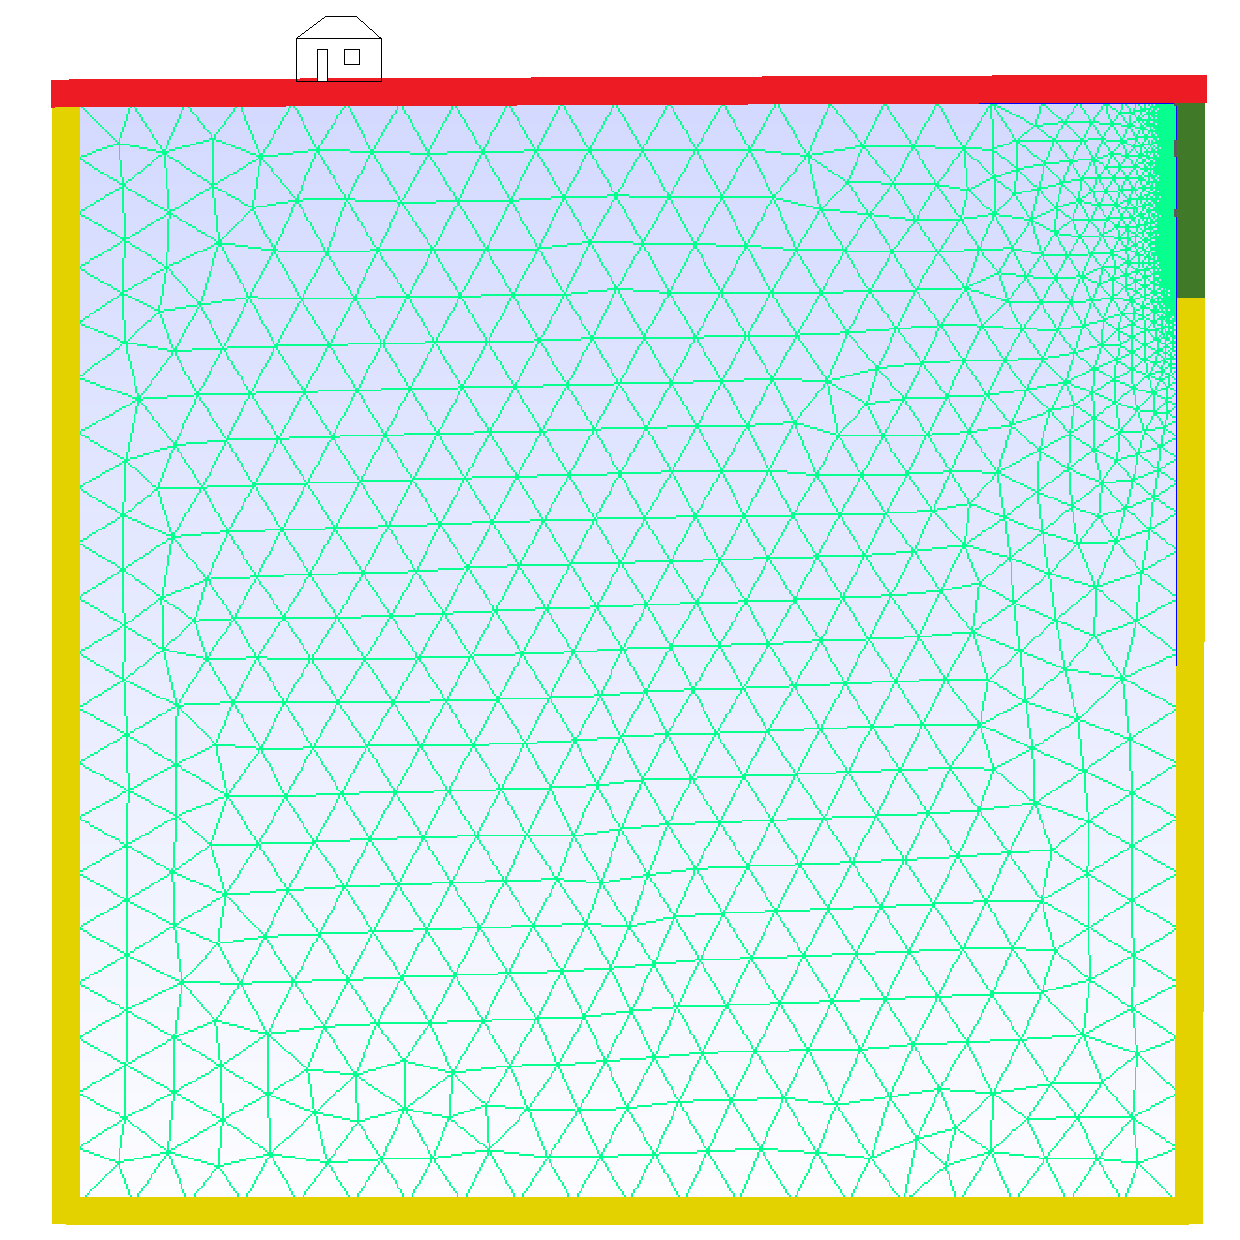
\includegraphics[width=0.4\textwidth]{images/BP1_mesh_with_boundaries.pdf}
	\caption{Space discretization of the BP1 problem with 200 elements on the fault}
	\label{fig:mesh_BP1_200_fault_elements}
\end{figure}

The elliptic Poisson problem $-\Delta u = f$ with mixed Dirichlet and Neumann boundary conditions is solved with the discontinuous Galerkin (DG) method described in \cite{DG-quick-tutorial}. First, the second order problem is transformed to a first order system, and after multiplication with test functions $\phi$ and $\varphi$ and integrating over a subset $K$ of $\Omega$ it is brought to the weak formulation in \autoref{eq:weakFormulationDG}.
\begin{equation}
	\label{eq:weakFormulationDG}
	\begin{cases}
		\;\;\ \int_K\nabla u\cdot\phi dV = -\int_Ku\nabla\cdot\phi dV + \int_{\partial K} u n_K\cdot\phi dS &\\
		\int_K\nabla u\cdot\nabla\varphi dV = \int_Kf\varphi dV + \int_{\partial K} \sigma\cdot n_K\varphi dS &
	\end{cases}
\end{equation} 
In the discretization, each element corresponds to such a subset $K$, the volume integrals stand than for the right hand side $f$ at the element and the surface integral for the numerical fluxes from one element to another or the boundary conditions if an element edge lies on the domain boundary. Dirichlet conditions are included with the penalty method as described in \cite{DG-elliptic-problems} and Neumann conditions can directly be added to the right-hand side of the second expression. If now the displacement $u$ in each element is represented as the weighted sum of basis functions, ... \\
To integrate an edge exactly with polynomial basis functions of order $k$, $k+1$ nodes are needed on the edge. In this thesis, we only consider the case $k=2$, so that the number of fault nodes is always three times the number of fault elements, and all relevant quantities for the time integration ($V$,$S$,$\psi$) are evaluated on these nodes. To obtain the displacement $u_i$ at each node in $\Omega$, a matrix $\mathbf{A}$, which combines the Gaussian integration weights with the gradients of the test functions, can be assembled such that:
\begin{equation}
	\mathbf{A}u = b(S)
\end{equation}
The matrix $\mathbf{A}$ does not depend on the displacement or any other variable, its LU-decomposition can therefore be calculated once at the beginning of the simulation and solving for the displacement only involves one forward and one backward substitution. The right-hand side $b$ includes all boundary conditions, especially from the slip at the rate-and-state fault, and therefore changes over time. 


\section{Evolution of Quantities}
\autoref{fig:EvolutionAllQuantitiesMinMaxStacked200Elements} gives a preview of the evolution of the characteristic quantities $S$, $\psi$ and $V$ in the rate-and-state fault. The maximum slip increases linearly over time, it corresponds to the bottom of the friction area in the fault, at the transition to the imposed slip rate. On the other hand, the minimum slip happens at the upper end, which remains constant until an earthquake suddenly shifts the open surface. Each earthquake is accompanied with a peak in the maximum slip rate up to $5$m/s, which usually remains below $10^{-9}$m/s in the aseismic phase. The state variable increases slowly until $0.8$ during the aseismic phase until an earthquake provokes a sudden drop to $0.4$. In the BP1 benchmark, an accurate prediction of the period between earthquakes is the most fundamental metric, this naturally implies an accurate evaluation of the aseismic phase but also of the earthquake, as the simulated slip increase at the open surface directly affects the duration to the next earthquake.

\begin{figure}[H]
	\centering
	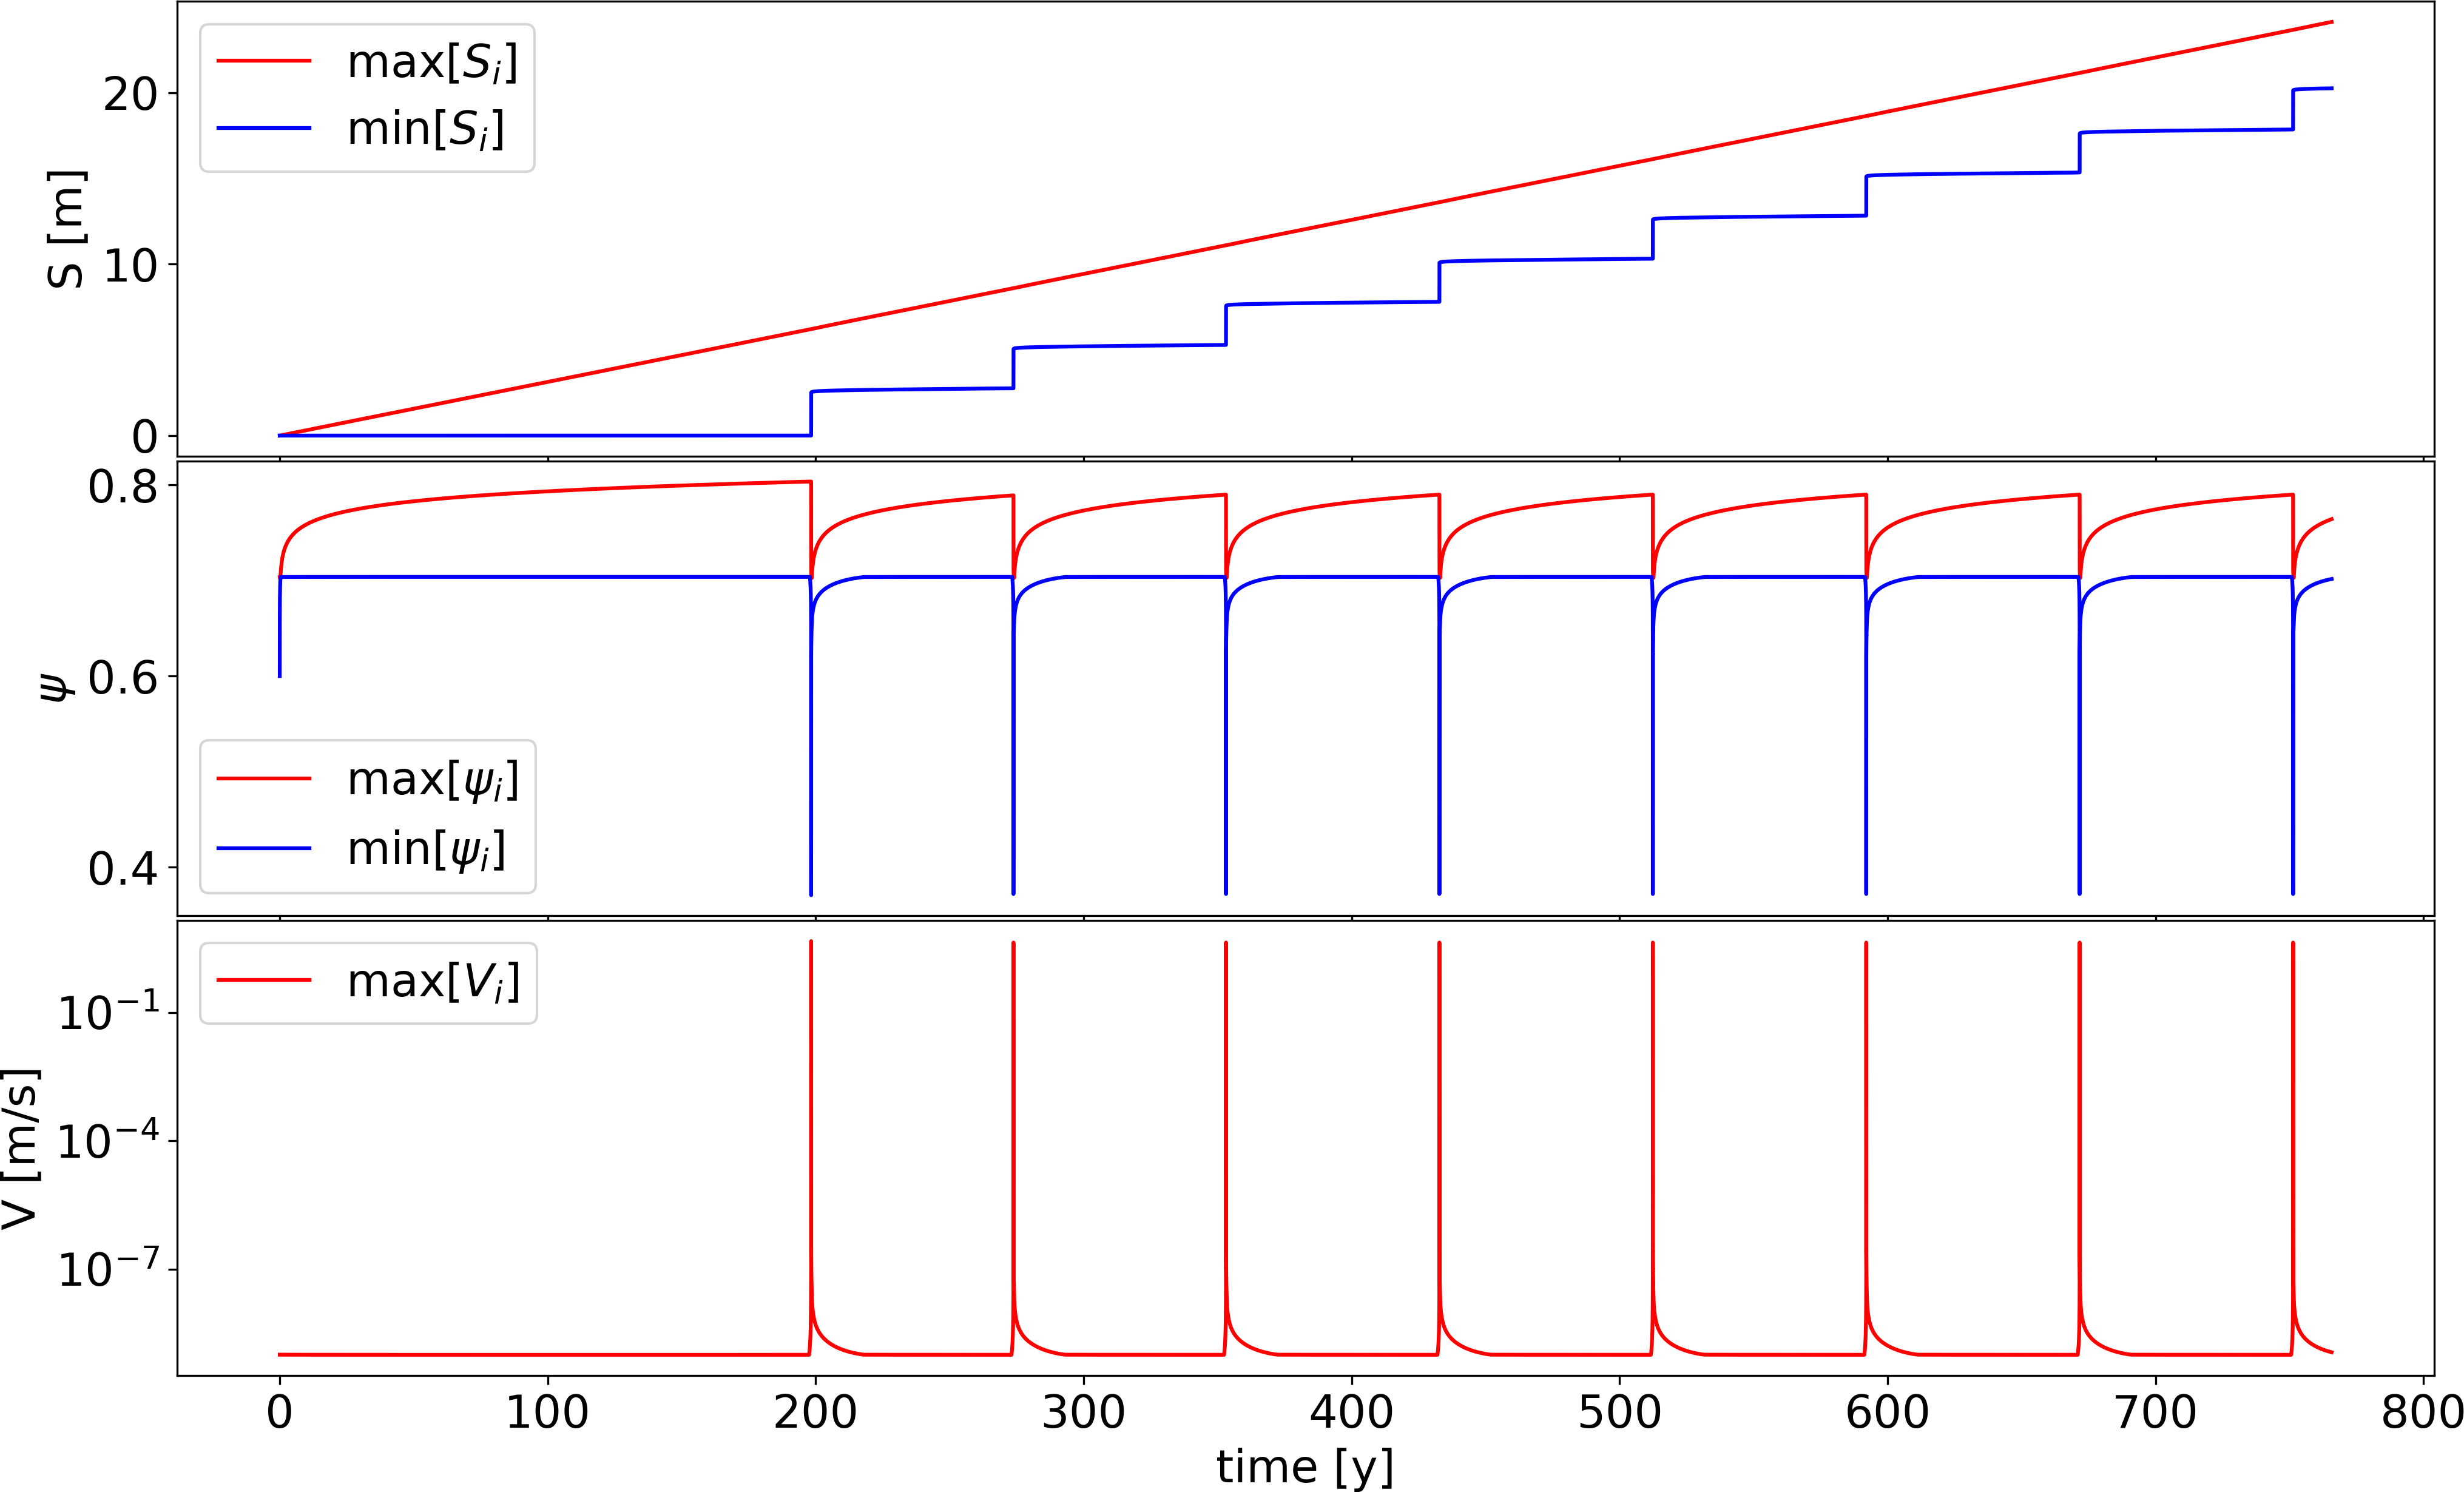
\includegraphics[width=0.7\textwidth]{images/TANDEMtimeEvolution_MinMaxAllStacked_Size200_RKDP5_extendedODE}
	\label{fig:EvolutionAllQuantitiesMinMaxStacked200Elements}
	\caption{Evolution of the slip $S$, the state variable $\psi$ and the slip rate $V$ over 770 years on a domain with 200 fault elements}
\end{figure}

A fine mesh resolution is essential for an accurate prediction of earthquake events. 
